\section{Durchführung}
\label{sec:Durchführung}

Für die Messung wurde eine Grundplatte wie in \autoref{fig:Abb1} dargestellt benutzt. Genauere Daten der Probestäbe wurden in der \autoref{tab:werte2} angegeben.

\begin{figure}
    \centering
    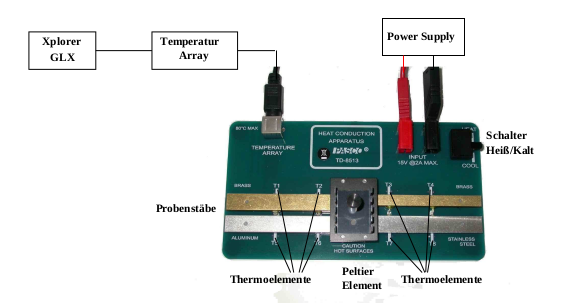
\includegraphics[scale=0.7]{content/Bilder/Aufbau.png}
    \caption{Hier zu sehen ist die für das Experiment verwendete Grundplatte, dessen Probestäbe im Verlauf des Versuchs aufgeheizt und abgekühlt wurden. Die einzelnen Bauteile sind hier beschrieben.}
    \label{fig:Abb1}
\end{figure}

\begin{table}
    \centering
    \caption{Hier ist eine Auflistung für die gegebenen Werte der Bauteile des Schwingkreises.}
    \label{tab:werte2}
    \begin{tabular}{c|c|c|c}
        Material & Abmessungen [cm] & $\rho$ [$\frac{kg}{m^3}$] & $c$ [$\frac{J}{kg\cdot K}$]\\
        \midrule
        Messing (breit) & 9 x 1.2 x 0.4 & 8520 & 385\\
        Messing (schmal) & 9 x 0.7 x 0.4 & 8520 & 385\\
        Aluminium & 9 x 1.2 x 0.4 & 2800 & 830\\
        Edelstahl & 9 x 1.2 x 0.4 & 8000 & 400\\
    \end{tabular}
  \end{table}

